\section{系统调用机制与中断}

中断是一种异步事件,它可以打断正在执行的程序并转移到处理中断的程序(中断处理程序)。
中断可以来自外部设备(如硬件中断)或软件(如系统调用)。中断机制是操作系统用来响应和处理中断的一种机制,
其中涉及中断向量表、中断控制器、中断处理程序等概念。

系统调用是中断的一种,通常情况下,U态的中断包括了系统调用,系统调用陷入内核态后,
将会调用SBI call来执行具体的内容。下面的\autoref{fig:syscall和SBI区别}清晰地展示了这两种中断的区别及联系。

\begin{figure}[htb]
    \centering
    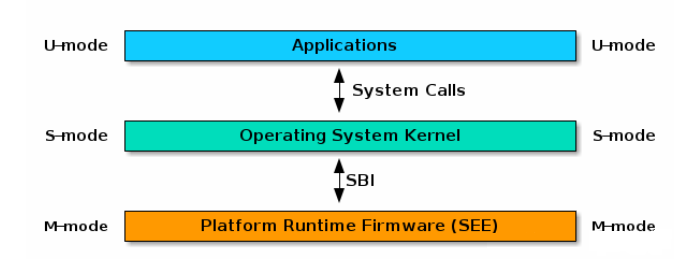
\includegraphics[width=\textwidth]{figures/03-03-syscall和SBI区别.png}
    \caption{
        syscall和SBI区别
    }
    \label{fig:syscall和SBI区别}
\end{figure}